
Model rankings are highly preserved between ImageNet and ImageNet-V2, with Kendall-$\tau$ = 0.9647. This exceeds the pre-registered threshold of 0.90, indicating that the original hypothesis of significant ranking shift is not supported.

\subsubsection{Main Results}

\begin{table}[htbp]
\centering
\resizebox{\columnwidth}{!}{%
\begin{tabular}{lll}
\toprule
Metric & Value & 95\% CI \\
\midrule
Kendall-$\tau$ & 0.9647 & [0.9454, 0.9795] \\
Spearman-$\rho$ & 0.9964 & --- \\
p-value & 1.58 $\times 10^{-43}$ & --- \\
\bottomrule
\end{tabular}
}
\end{table}

The observed $\tau$ = 0.9647 indicates near-perfect ranking preservation. The 95\% confidence interval [0.9454, 0.9795] lies entirely above the 0.90 threshold. Spearman-$\rho$ = 0.9964 confirms this finding.

\begin{figure}[htbp]
\centering
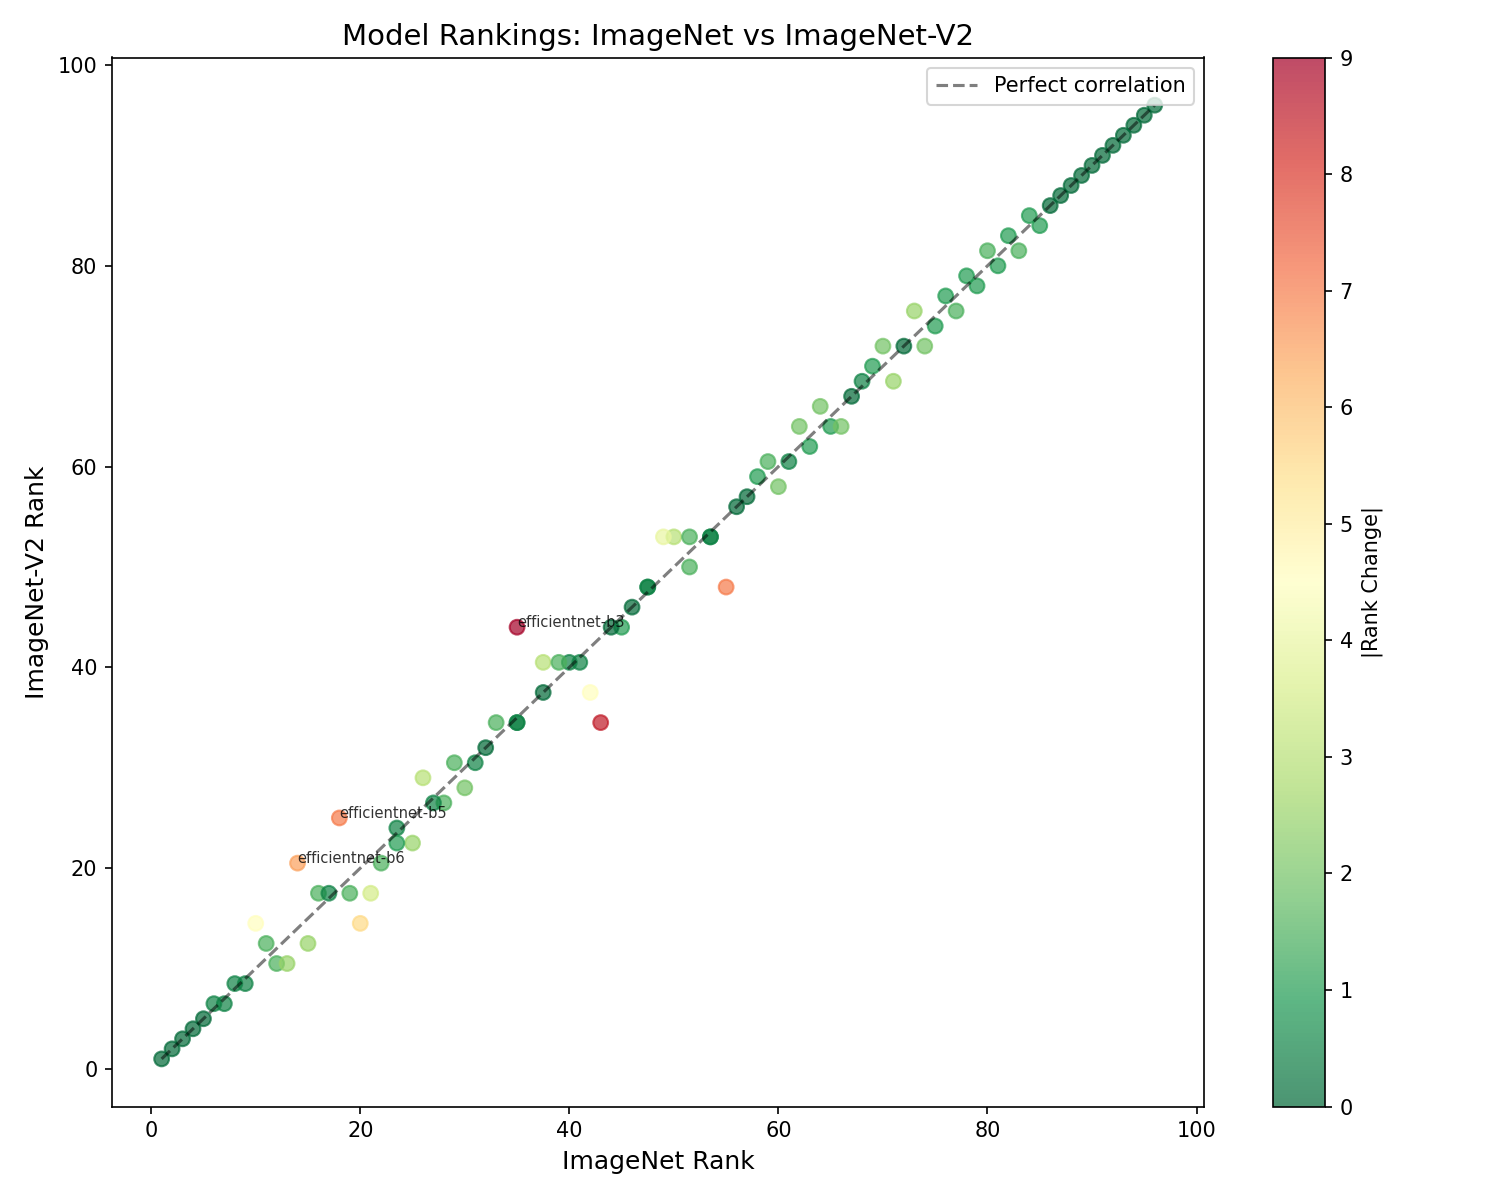
\includegraphics[width=\columnwidth]{figures/ranking_scatter.png}
\caption{Figure 1: Ranking scatter plot}
\label{fig:ranking_scatter}
\end{figure}
\textit{Figure 1: ImageNet rank vs. ImageNet-V2 rank for 96 models. Points along the diagonal indicate ranking preservation ($\tau$ = 0.9647).}

\subsubsection{Accuracy Degradation Analysis}

Despite ranking stability, models experience substantial accuracy drops on ImageNet-V2:

\begin{table}[htbp]
\centering
\resizebox{\columnwidth}{!}{%
\begin{tabular}{ll}
\toprule
Statistic & Value \\
\midrule
Mean accuracy drop & 11.68\% \\
Median accuracy drop & 11.52\% \\
Standard deviation & 1.87\% \\
Min drop & 7.4\% \\
Max drop & 16.2\% \\
\bottomrule
\end{tabular}
}
\end{table}

Accuracy drops are substantial (~12\% on average) but remarkably uniform across models. This uniformity explains ranking preservation: when all models lose similar percentages, their relative ordering remains unchanged.

\begin{figure}[htbp]
\centering
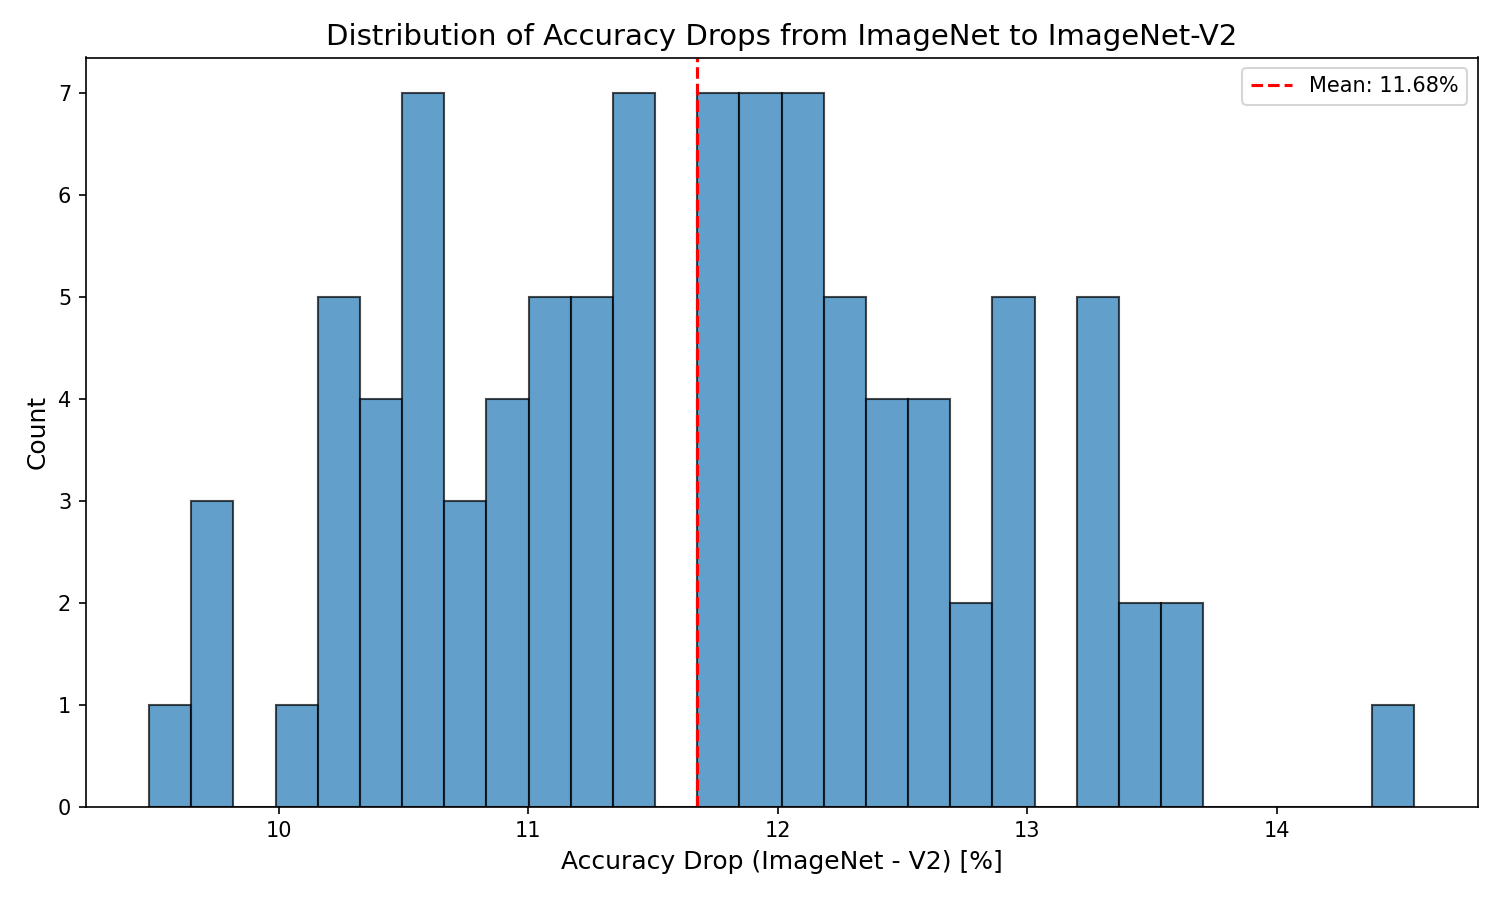
\includegraphics[width=\columnwidth]{figures/accuracy_drop.png}
\caption{Figure 2: Accuracy drop distribution}
\label{fig:accuracy_drop}
\end{figure}
\textit{Figure 2: Distribution of accuracy drops from ImageNet to ImageNet-V2. The narrow spread (SD = 1.87\%) indicates uniform degradation across models.}

\subsubsection{Rank Change Analysis}

\begin{table}[htbp]
\centering
\resizebox{\columnwidth}{!}{%
\begin{tabular}{ll}
\toprule
Statistic & Value \\
\midrule
Mean rank change & 2.8 positions \\
Median rank change & 2 positions \\
Max rank change & 9 positions \\
Models with no rank change & 8 (8.3\%) \\
Models with $\leq 3$ position change & 72 (75\%) \\
\bottomrule
\end{tabular}
}
\end{table}

\begin{figure}[htbp]
\centering
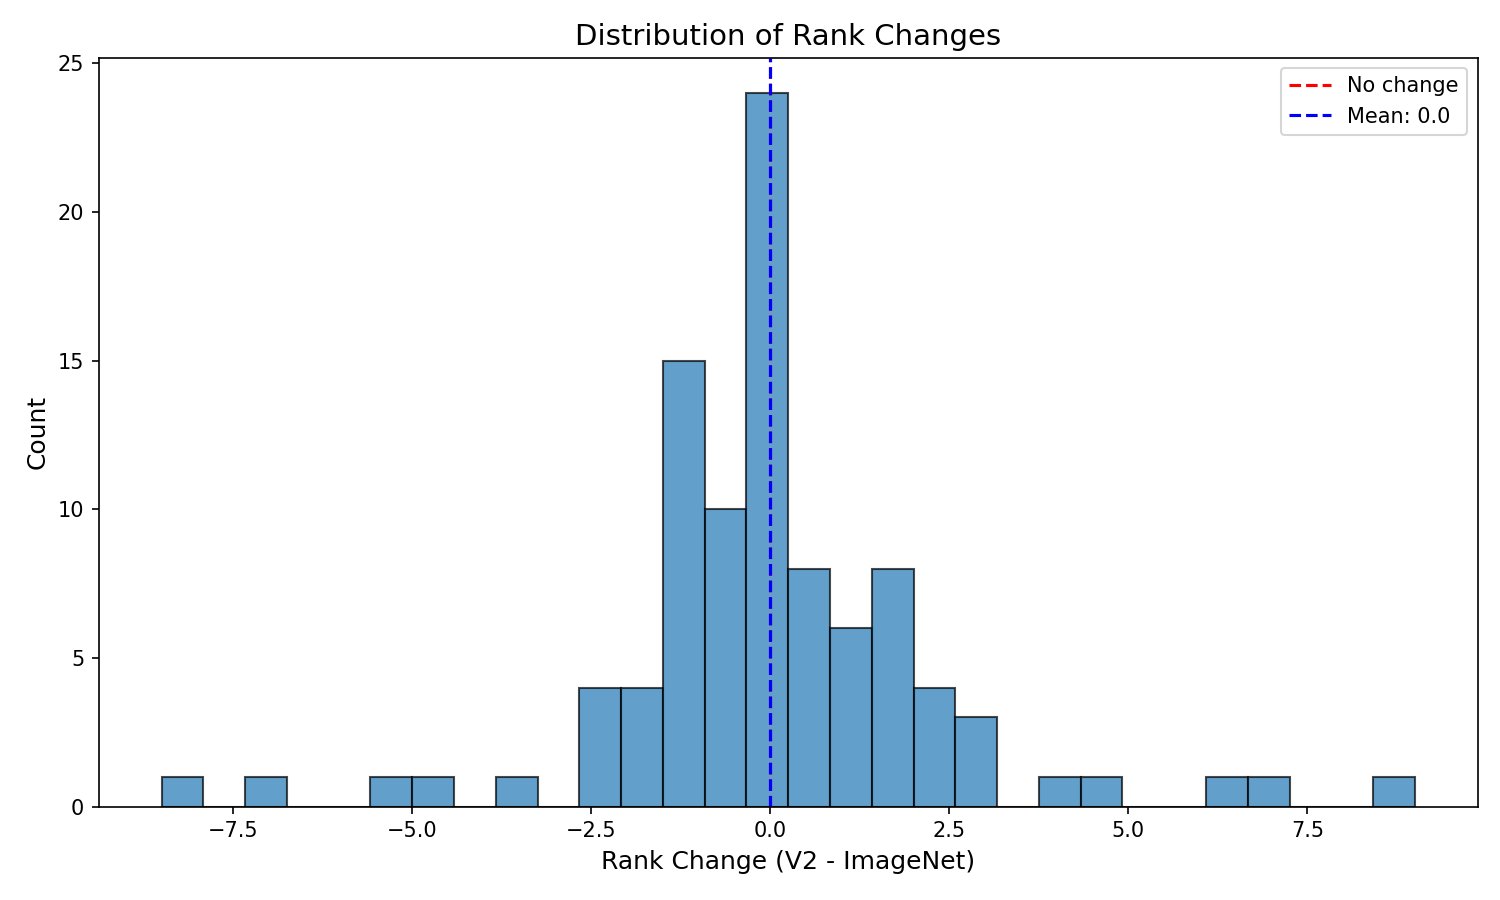
\includegraphics[width=\columnwidth]{figures/rank_change_distribution.png}
\caption{Figure 3: Rank change distribution}
\label{fig:rank_change_distribution}
\end{figure}
\textit{Figure 3: Distribution of rank changes. 75\% of models change by $\leq 3$ positions; maximum change is 9.}

\subsubsection{Gate Evaluation}

The pre-registered criterion ($\tau$ < 0.90) was not met:

\begin{table}[htbp]
\centering
\resizebox{\columnwidth}{!}{%
\begin{tabular}{llll}
\toprule
Metric & Threshold & Actual & Status \\
\midrule
Kendall-$\tau$ & < 0.90 & 0.9647 & NOT MET \\
p-value & < 0.001 & 1.58e-43 & MET \\
\bottomrule
\end{tabular}
}
\end{table}

